\documentclass[
  shownotes,
  xcolor={svgnames},
  hyperref={colorlinks,citecolor=DarkBlue,linkcolor=andesred,urlcolor=DarkBlue}
  , aspectratio=169]{beamer}
\usepackage{animate}
\usepackage{amsmath}
\usepackage{amsfonts}
\usepackage{amssymb}
\usepackage{pifont}
\usepackage{mathpazo}
%\usepackage{xcolor}
\usepackage{multimedia}
\usepackage{fancybox}
\usepackage[para]{threeparttable}
\usepackage{multirow}
\setcounter{MaxMatrixCols}{30}
\usepackage{subcaption}
\usepackage{graphicx}
\usepackage{lscape}
\usepackage[compatibility=false,font=small]{caption}
\usepackage{booktabs}
\usepackage{ragged2e}
\usepackage{chronosys}
\usepackage{appendixnumberbeamer}
\usepackage{animate}
\setbeamertemplate{caption}[numbered]
\usepackage{color}
%\usepackage{times}
\usepackage{tikz}
\usetikzlibrary{arrows}
\usepackage{comment} %to comment
%% BibTeX settings
\usepackage{natbib}
\bibliographystyle{apalike}
\bibpunct{(}{)}{,}{a}{,}{,}
\setbeamertemplate{bibliography item}{[\theenumiv]}

% Defines columns for bespoke tables
\usepackage{array}
\newcolumntype{L}[1]{>{\raggedright\let\newline\\\arraybackslash\hspace{0pt}}m{#1}}
\newcolumntype{C}[1]{>{\centering\let\newline\\\arraybackslash\hspace{0pt}}m{#1}}
\newcolumntype{R}[1]{>{\raggedleft\let\newline\\\arraybackslash\hspace{0pt}}m{#1}}


\usepackage{xfrac}


\usepackage{multicol}
\setlength{\columnsep}{0.5cm}

% Theme and colors
\usetheme{Boadilla}

% I define a custom pallete
\definecolor{andesred}{HTML}{1B175E}
\definecolor{andesyellow}{HTML}{ffff00}

% Other options
\providecommand{\U}[1]{\protect\rule{.1in}{.1in}}
\usefonttheme{serif}
\setbeamertemplate{itemize items}[default]
\setbeamertemplate{enumerate items}[square]
\setbeamertemplate{section in toc}[circle]


\definecolor{mybackground}{HTML}{1B175E}
\definecolor{myforeground}{HTML}{0000A0}

\setbeamercolor{normal text}{fg=black,bg=white}
\setbeamercolor{alerted text}{fg=andesred}
\setbeamercolor{example text}{fg=black}

\setbeamercolor{background canvas}{fg=myforeground, bg=white}
\setbeamercolor{background}{fg=myforeground, bg=mybackground}
\setbeamercolor{palette tertiary}{fg=myforeground,bg=mybackground}

\setbeamercolor{palette primary}{fg=black, bg=white}
\setbeamercolor{palette secondary}{fg=black, bg=white!10!andesyellow}
\setbeamercolor{palette tertiary}{fg=black, bg=white}


\setbeamercolor{frametitle}{fg=black}
\setbeamercolor{title}{fg=black}
\setbeamercolor{block title}{fg=andesred}
\setbeamercolor{itemize item}{fg=andesred}
\setbeamercolor{itemize subitem}{fg=andesred}
\setbeamercolor{itemize subsubitem}{fg=andesred}
\setbeamercolor{enumerate item}{fg=andesred}
\setbeamercolor{item projected}{bg=gray!30!white,fg=andesred}
\setbeamercolor{enumerate subitem}{fg=andesred}
\setbeamercolor{section number projected}{bg=gray!30!white,fg=andesred}
\setbeamercolor{section in toc}{fg=andesred}
\setbeamercolor{caption name}{fg=andesred}
\setbeamercolor{button}{bg=gray!30!white,fg=andesred}
\setbeamercolor{title in head/foot}{fg=andesred}



\usepackage{fancyvrb}
\newcommand{\VerbBar}{|}
\newcommand{\VERB}{\Verb[commandchars=\\\{\}]}
\DefineVerbatimEnvironment{Highlighting}{Verbatim}{commandchars=\\\{\}}
% Add ',fontsize=\small' for more characters per line
\usepackage{framed}
\definecolor{shadecolor}{RGB}{248,248,248}
\newenvironment{Shaded}{\begin{snugshade}}{\end{snugshade}}
\newcommand{\AlertTok}[1]{\textcolor[rgb]{0.94,0.16,0.16}{#1}}
\newcommand{\AnnotationTok}[1]{\textcolor[rgb]{0.56,0.35,0.01}{\textbf{\textit{#1}}}}
\newcommand{\AttributeTok}[1]{\textcolor[rgb]{0.77,0.63,0.00}{#1}}
\newcommand{\BaseNTok}[1]{\textcolor[rgb]{0.00,0.00,0.81}{#1}}
\newcommand{\BuiltInTok}[1]{#1}
\newcommand{\CharTok}[1]{\textcolor[rgb]{0.31,0.60,0.02}{#1}}
\newcommand{\CommentTok}[1]{\textcolor[rgb]{0.56,0.35,0.01}{\textit{#1}}}
\newcommand{\CommentVarTok}[1]{\textcolor[rgb]{0.56,0.35,0.01}{\textbf{\textit{#1}}}}
\newcommand{\ConstantTok}[1]{\textcolor[rgb]{0.00,0.00,0.00}{#1}}
\newcommand{\ControlFlowTok}[1]{\textcolor[rgb]{0.13,0.29,0.53}{\textbf{#1}}}
\newcommand{\DataTypeTok}[1]{\textcolor[rgb]{0.13,0.29,0.53}{#1}}
\newcommand{\DecValTok}[1]{\textcolor[rgb]{0.00,0.00,0.81}{#1}}
\newcommand{\DocumentationTok}[1]{\textcolor[rgb]{0.56,0.35,0.01}{\textbf{\textit{#1}}}}
\newcommand{\ErrorTok}[1]{\textcolor[rgb]{0.64,0.00,0.00}{\textbf{#1}}}
\newcommand{\ExtensionTok}[1]{#1}
\newcommand{\FloatTok}[1]{\textcolor[rgb]{0.00,0.00,0.81}{#1}}
\newcommand{\FunctionTok}[1]{\textcolor[rgb]{0.00,0.00,0.00}{#1}}
\newcommand{\ImportTok}[1]{#1}
\newcommand{\InformationTok}[1]{\textcolor[rgb]{0.56,0.35,0.01}{\textbf{\textit{#1}}}}
\newcommand{\KeywordTok}[1]{\textcolor[rgb]{0.13,0.29,0.53}{\textbf{#1}}}
\newcommand{\NormalTok}[1]{#1}
\newcommand{\OperatorTok}[1]{\textcolor[rgb]{0.81,0.36,0.00}{\textbf{#1}}}
\newcommand{\OtherTok}[1]{\textcolor[rgb]{0.56,0.35,0.01}{#1}}
\newcommand{\PreprocessorTok}[1]{\textcolor[rgb]{0.56,0.35,0.01}{\textit{#1}}}
\newcommand{\RegionMarkerTok}[1]{#1}
\newcommand{\SpecialCharTok}[1]{\textcolor[rgb]{0.00,0.00,0.00}{#1}}
\newcommand{\SpecialStringTok}[1]{\textcolor[rgb]{0.31,0.60,0.02}{#1}}
\newcommand{\StringTok}[1]{\textcolor[rgb]{0.31,0.60,0.02}{#1}}
\newcommand{\VariableTok}[1]{\textcolor[rgb]{0.00,0.00,0.00}{#1}}
\newcommand{\VerbatimStringTok}[1]{\textcolor[rgb]{0.31,0.60,0.02}{#1}}
\newcommand{\WarningTok}[1]{\textcolor[rgb]{0.56,0.35,0.01}{\textbf{\textit{#1}}}}
\usepackage{graphicx}
\makeatletter

\makeatother


\AtBeginSection[]
{
    \begin{frame}
        \frametitle{Agenda}
        \tableofcontents[currentsection]
    \end{frame}
}



\AtBeginSubsection[]
{
    \begin{frame}
        \frametitle{Agenda}
        \tableofcontents[currentsubsection]
    \end{frame}
}





%%%%%%%%%%%%%%% BEGINS DOCUMENT %%%%%%%%%%%%%%%%%%



\begin{document}

\title{Classification}
\subtitle{Big Data y Machine Learning para Economía Aplicada}
\date{}

\author[Sarmiento-Barbieri]{Ignacio Sarmiento-Barbieri}
\institute[Uniandes]{Universidad de los Andes}


\begin{frame}[noframenumbering]
\maketitle
\end{frame}


%----------------------------------------------------------------------%
%----------------------------------------------------------------------%
\section{Motivation}
%----------------------------------------------------------------------%
%----------------------------------------------------------------------%
\begin{frame}[fragile]
\frametitle{Classification: Motivation}

\begin{itemize}
  \item Many predictive questions are about classification
  \medskip
  \begin{itemize}
      \item Email should go to the spam folder or not
      \medskip
      \item A household is bellow the poverty line
      \medskip
      \item Accept someone to a graduate program or no
      \medskip
      \end{itemize}
\item Aim is to classify $y$ based on $X's$

\end{itemize}
\end{frame}
%----------------------------------------------------------------------%
\begin{frame}[fragile]
\frametitle{Classification: Motivation}

\begin{itemize}
\item Main difference is that $y$ represents membership in a category: $y\in \{1,2,...,n\}$
\medskip
\begin{itemize}
  \item Qualitative (e.g., spam, personal, social)
  \medskip
  \item Not necessarily ordered
  
\end{itemize}
\bigskip
  \begin{center}
    \begin{it}
    \large
      The prediction question is, given a new $X$, \\
      what is our best guess at the response category $\hat{y}$
    \end{it}
  \end{center}
\end{itemize}


\end{frame}
%----------------------------------------------------------------------%
%----------------------------------------------------------------------%
\section{Risk, Probability, and Classification}
%----------------------------------------------------------------------%
%----------------------------------------------------------------------%
\begin{frame}[fragile]
\frametitle{Risk, Probability, and Classification}

\begin{itemize}
  \item Two states of nature $Y \rightarrow i\in\{0,1\}$
  \medskip
  \item Two actions $(\hat{Y}) \rightarrow j\in \{0,1\}$
\end{itemize}

\begin{table}[H]
\centering
\begin{tabular}{cc|cc}
& \multicolumn{3}{c}{$\hat{Y}$}\tabularnewline
&  & 0 & 1 \\[5pt]
\hline\\[5pt]
\multirow{2}{*}{Y} & 0 & True Negative & False Positive \\[10pt]
& 1 & False Negative & True Positive \\
\end{tabular}
\end{table}
\end{frame}
%----------------------------------------------------------------------%
\begin{frame}[fragile]
\frametitle{Risk, Probability, and Classification}

        \begin{figure}[H] \centering
            \captionsetup{justification=centering}
              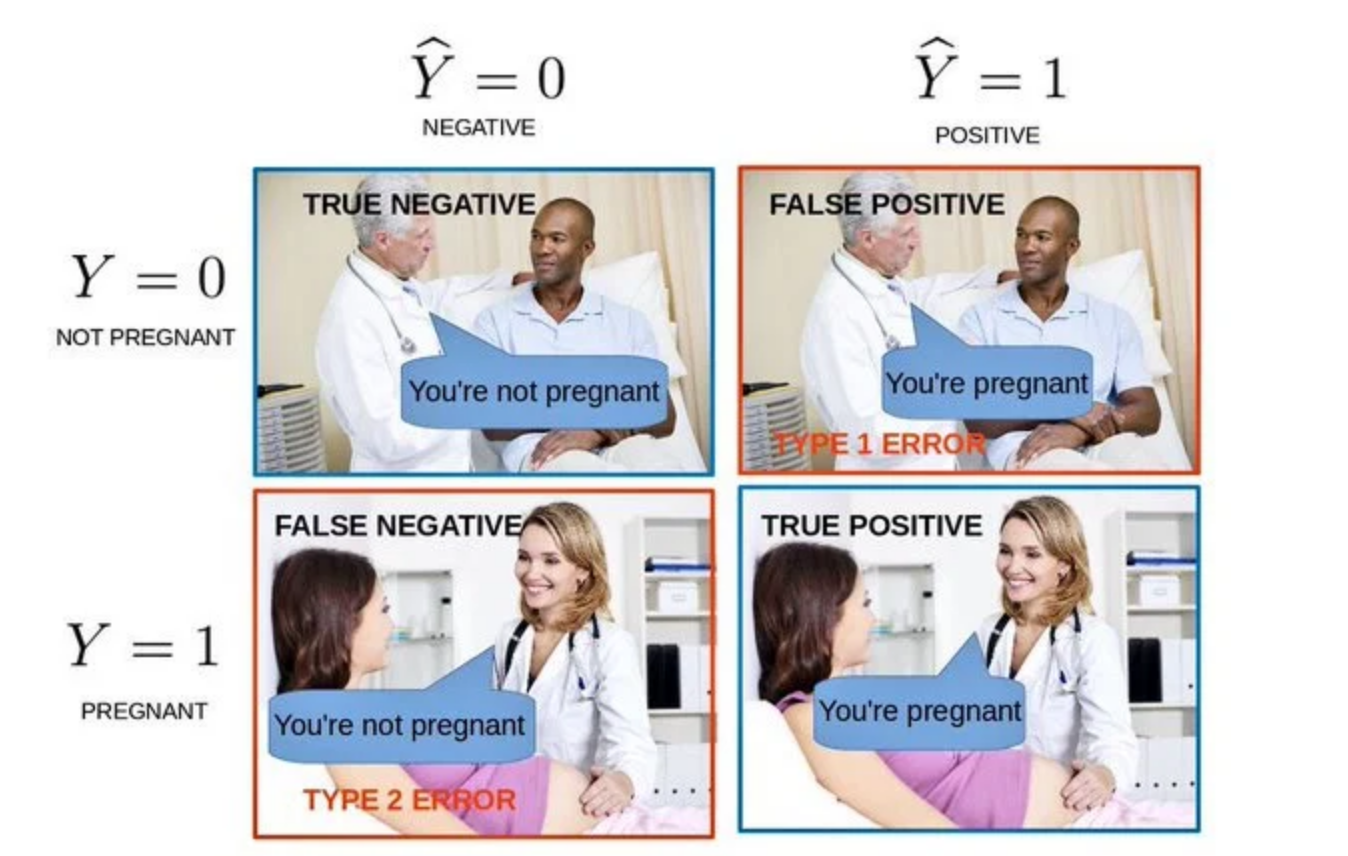
\includegraphics[scale=0.4]{figures/confusion_matrix}
              \\
              \tiny
              Source: \url{https://dzone.com/articles/understanding-the-confusion-matrix}
 \end{figure}

  
\end{frame}
%----------------------------------------------------------------------%
\begin{frame}[fragile]
\frametitle{Risk, Probability, and Classification}

\begin{itemize}
  \item Two actions $\hat{Y} \rightarrow j\in \{0,1\}$
  \medskip
  \item Two states of nature $Y \rightarrow i\in\{0,1\}$
  \medskip
  
  \item Probabilities
  \medskip
  \begin{itemize}
    \item $p=Pr(Y=1|X)$
    \medskip
    \item $1-p=Pr(Y=0|X)$
  \end{itemize}
  \end{itemize}

\end{frame}
%----------------------------------------------------------------------%
\begin{frame}[fragile]
\frametitle{Risk, Probability, and Classification}

\begin{itemize}
  \item Actions have costs associated to them

  \medskip
  \item Loss: $L(i,j)$, penalizes being in bin $i,j$
\begin{itemize}
  
  \medskip
  \item We define $L(i,j)$
  \medskip
        \begin{align}
        L(i,j)=\begin{cases}
                  1 & i\neq j\\
                  0 & i=j
                \end{cases}
        \end{align}
\end{itemize}
\end{itemize}

  \end{frame}
%----------------------------------------------------------------------%
\begin{frame}[fragile]
\frametitle{Risk, Probability, and Classification}
\begin{itemize}
  \item Risk: expected loss of taking action $j$
  
  \medskip

\begin{align}
E[L(i,j)] &= \sum_i p_j L(i,j) \\ \nonumber
R(j) &= (1-p) L(0,j) + p L(1,j)
\end{align}

\medskip
  \item The objective is to minimize the risk
\end{itemize}





\end{frame}
%----------------------------------------------------------------------%
%----------------------------------------------------------------------%
\section{Bayes Classifier}
%----------------------------------------------------------------------%
%----------------------------------------------------------------------%

\begin{frame}[fragile]
\frametitle{Bayes classifier}

\begin{eqnarray}
R(1) &< R(0)  \\[10pt] \nonumber \pause
1-p &< p \\[10pt] \nonumber \pause
p &> \frac{1}{2} \\ \nonumber
\end{eqnarray}


\end{frame}
%----------------------------------------------------------------------%
\begin{frame}[fragile]
\frametitle{Bayes classifier}

\begin{itemize}
  \item Under a 0-1 penalty the problem boils down to finding 

\begin{align}
p=Pr(Y=1|X)
\end{align}
  
  \medskip
  \item We then predict 1 if $p>0.5$ and 0 otherwise (Bayes classifier)
  \medskip
  \item Many ways of finding this probability in binary cases
\end{itemize}


\end{frame}
%----------------------------------------------------------------------%
%----------------------------------------------------------------------%
\section{Logit}
%----------------------------------------------------------------------%
%----------------------------------------------------------------------%

%----------------------------------------------------------------------%
\begin{frame}[fragile]
\frametitle{Setup}


\begin{itemize}

  \item  $Y$ is a binary random variable$\{0,1\}$
  \medskip
  \item $X$ is a vector of K predictors
  \medskip
  
  \item $p=Pr(Y=1|X)$
  
  \end{itemize}

\end{frame}
%----------------------------------------------------------------------%
\begin{frame}[fragile]
\frametitle{Logit}



        \begin{figure}[H] \centering
            \captionsetup{justification=centering}
              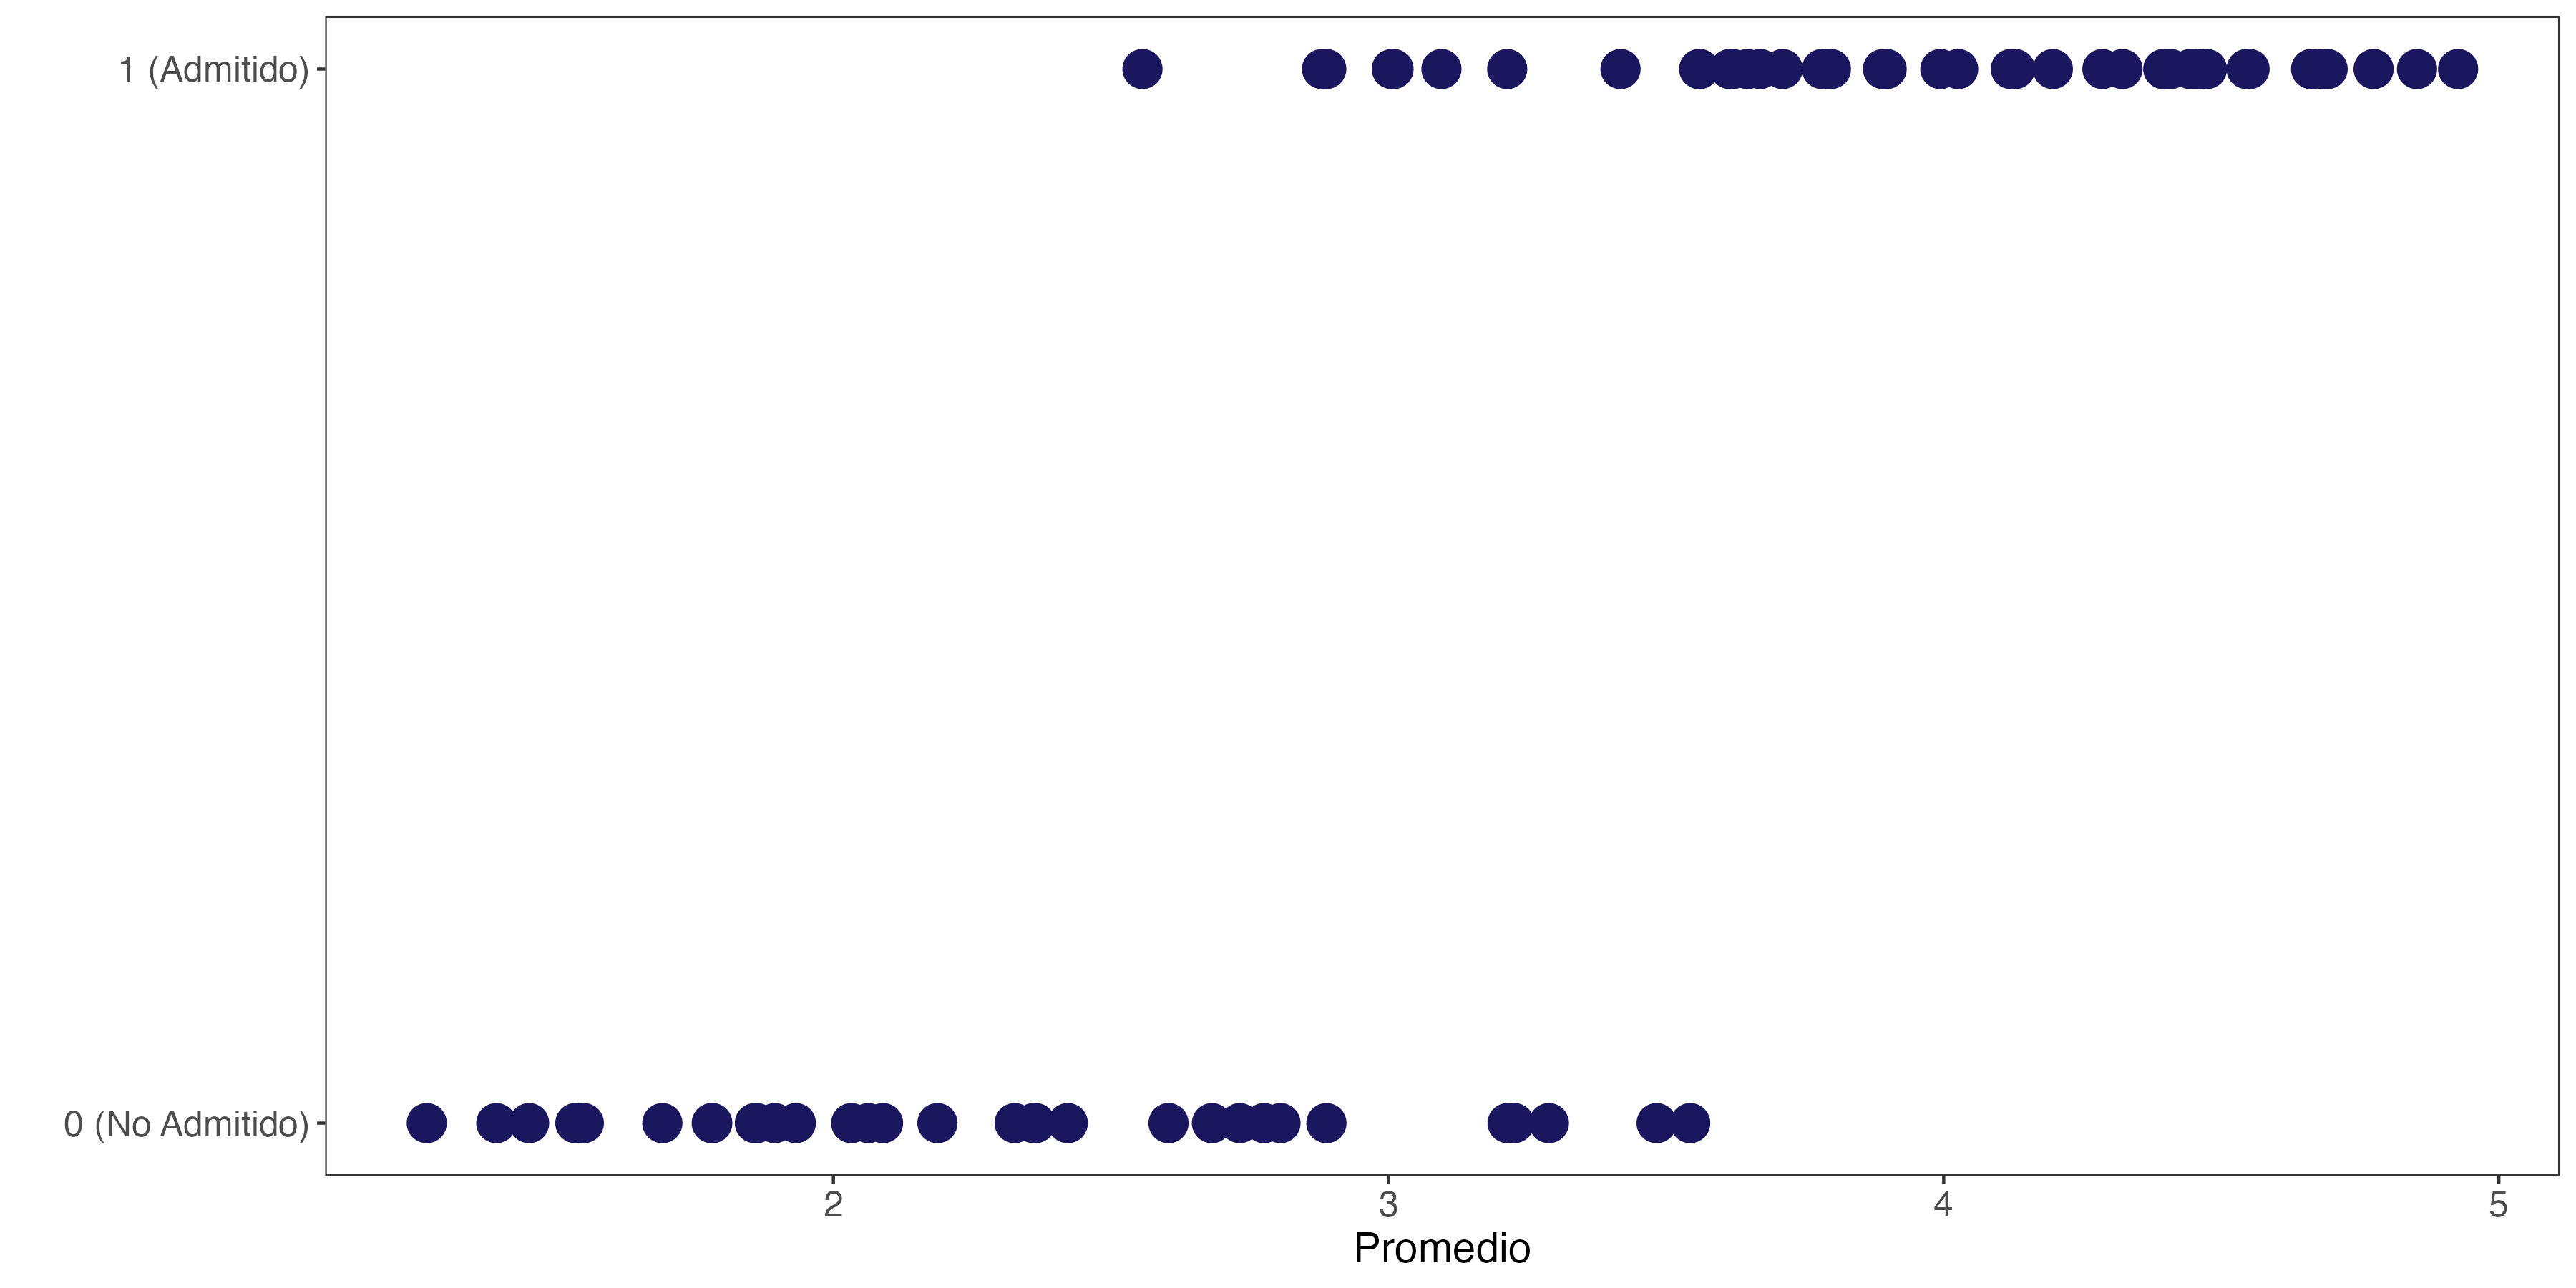
\includegraphics[scale=0.45]{figures/fig1}
              
 \end{figure}


\end{frame}
%----------------------------------------------------------------------%
\begin{frame}[fragile]
\frametitle{Logit}



        \begin{figure}[H] \centering
            \captionsetup{justification=centering}
              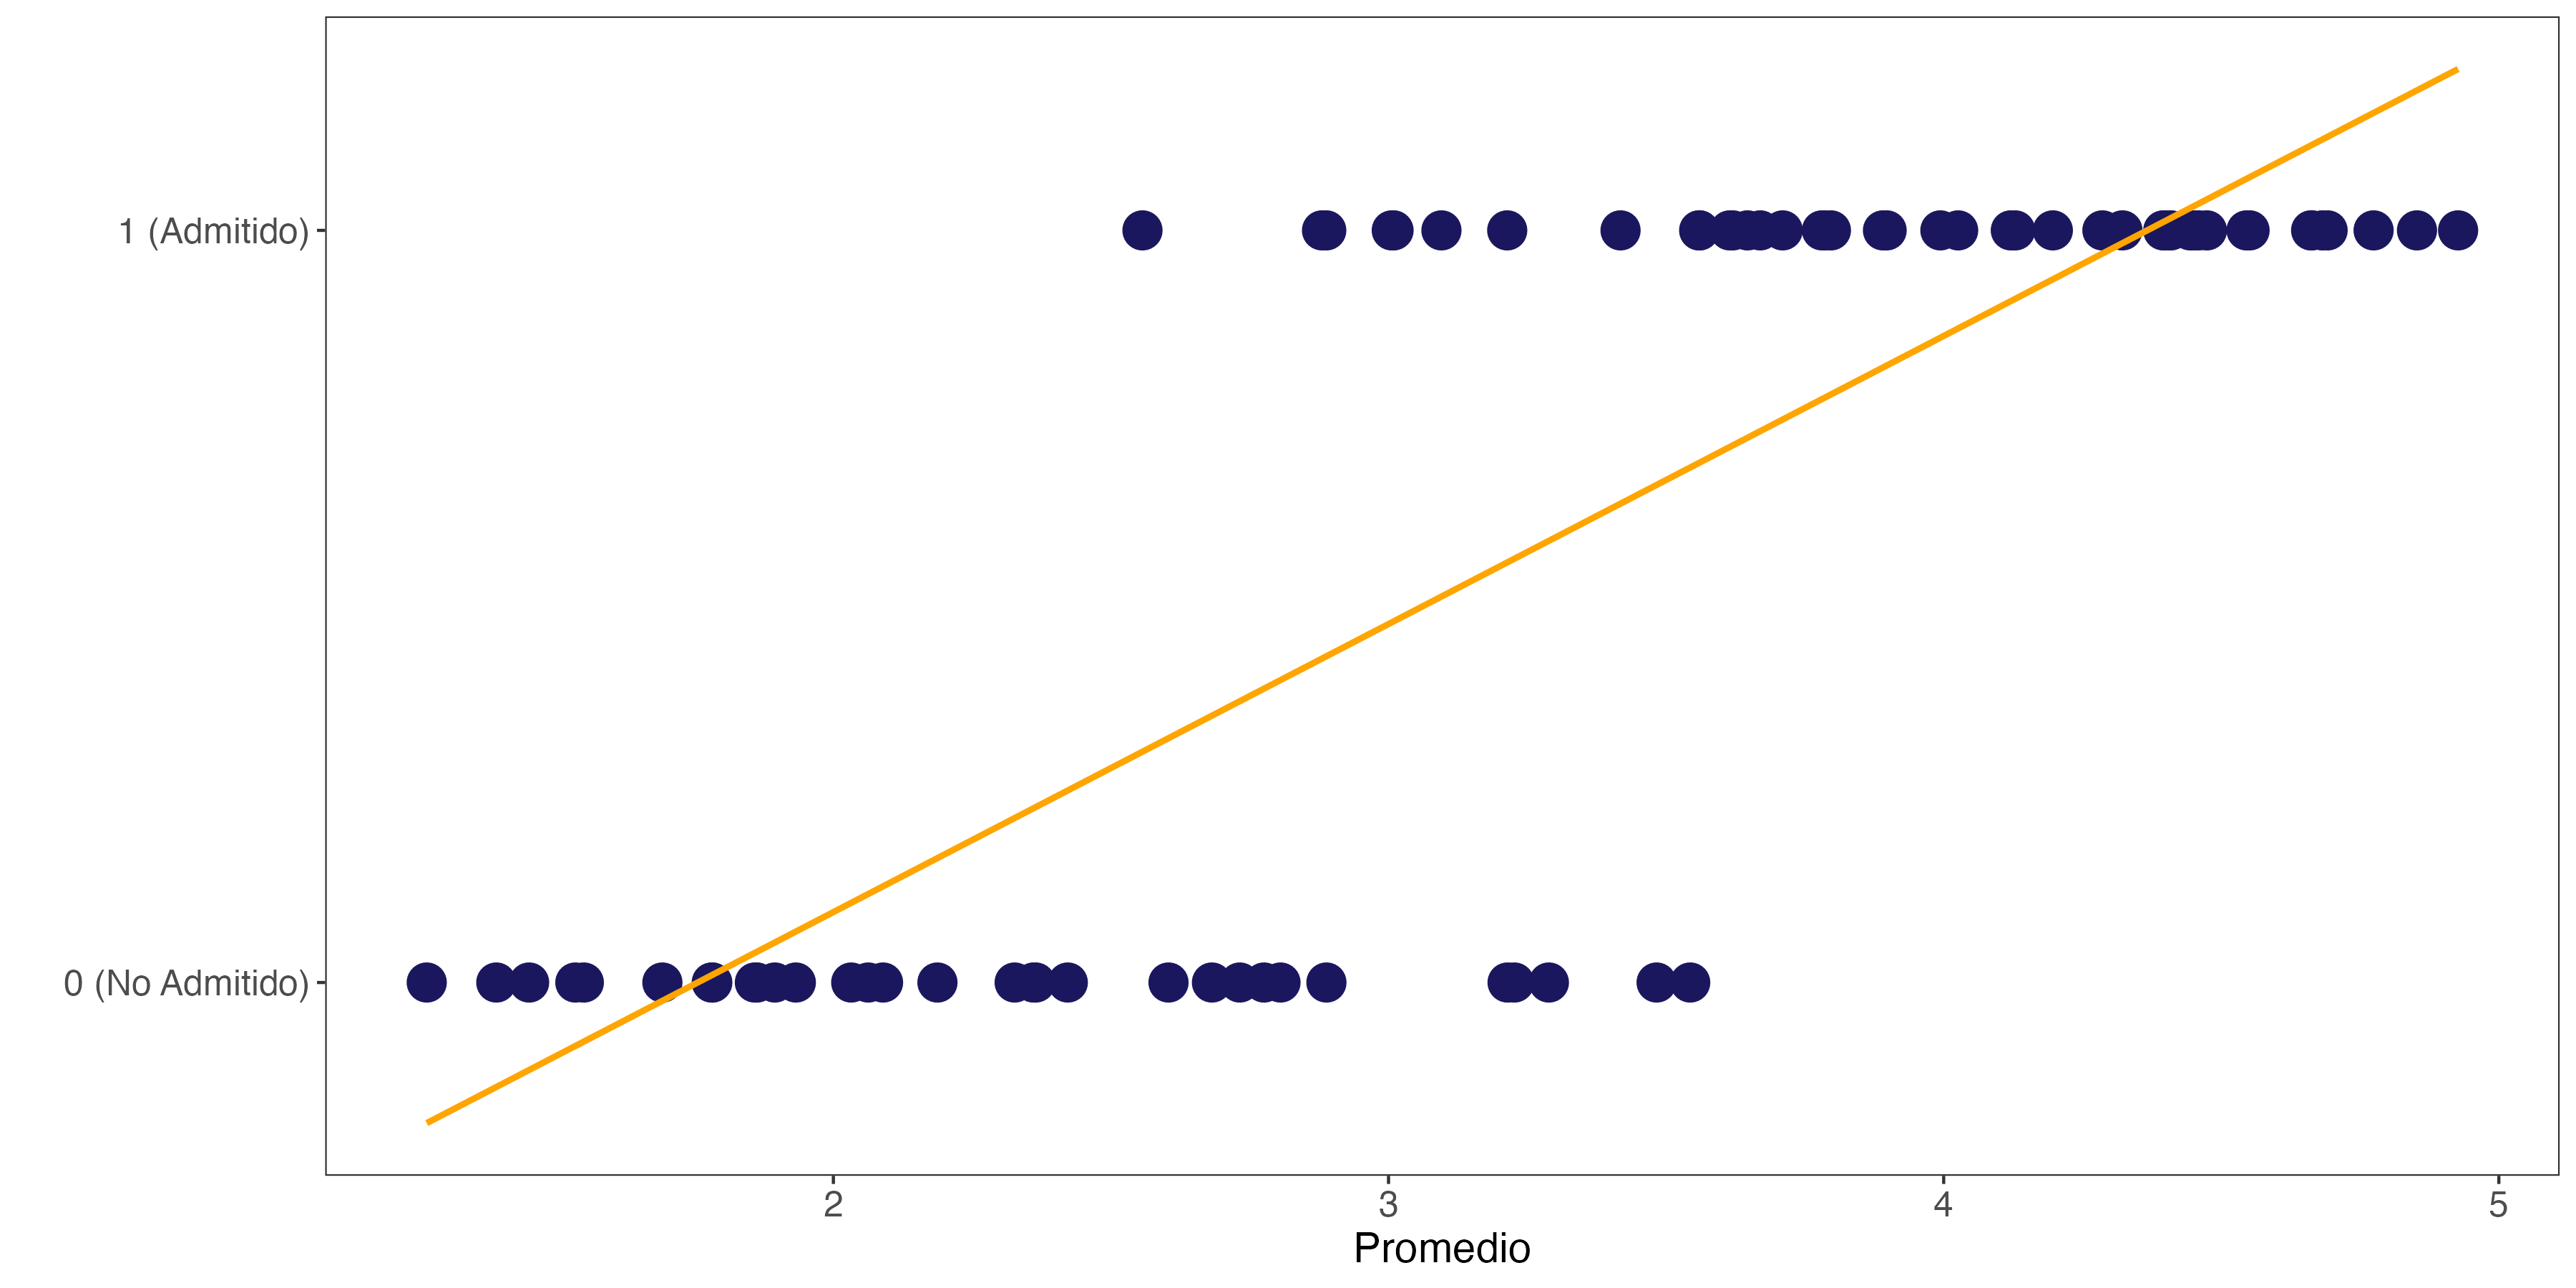
\includegraphics[scale=0.45]{figures/fig2}
              
 \end{figure}



\end{frame}
%----------------------------------------------------------------------%
\begin{frame}[fragile]
\frametitle{Logit}



        \begin{figure}[H] \centering
            \captionsetup{justification=centering}
              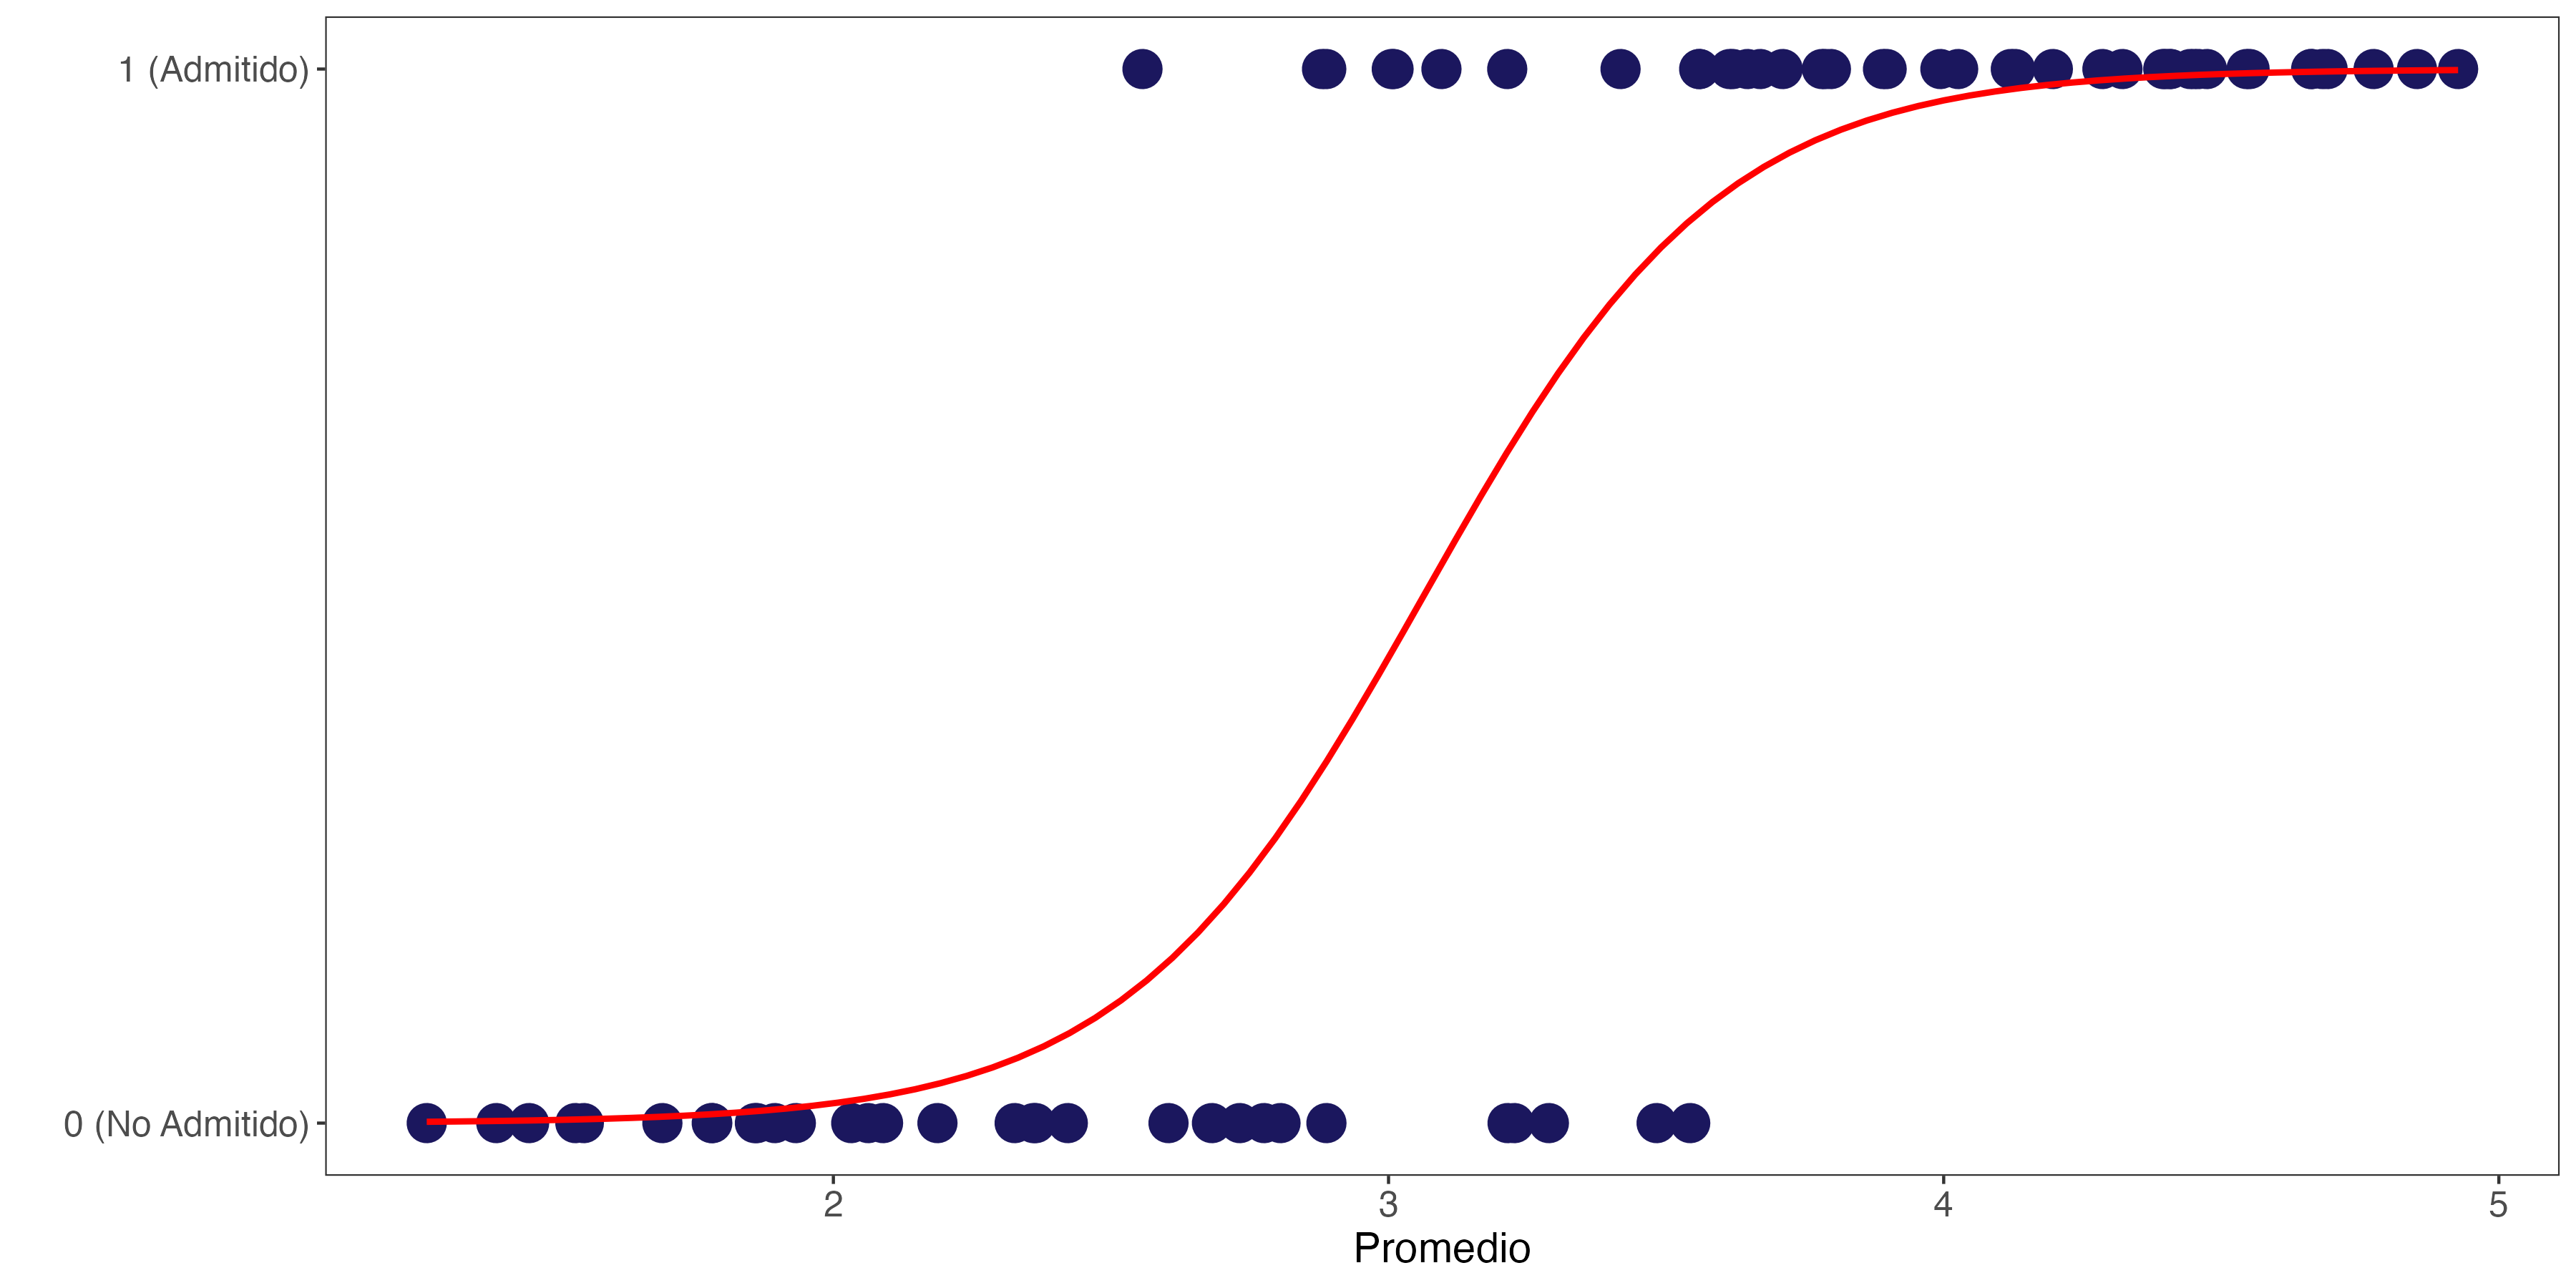
\includegraphics[scale=0.45]{figures/fig3}
              
 \end{figure}



\end{frame}
%----------------------------------------------------------------------%
\begin{frame}[fragile]
\frametitle{Logit}



        \begin{figure}[H] \centering
            \captionsetup{justification=centering}
              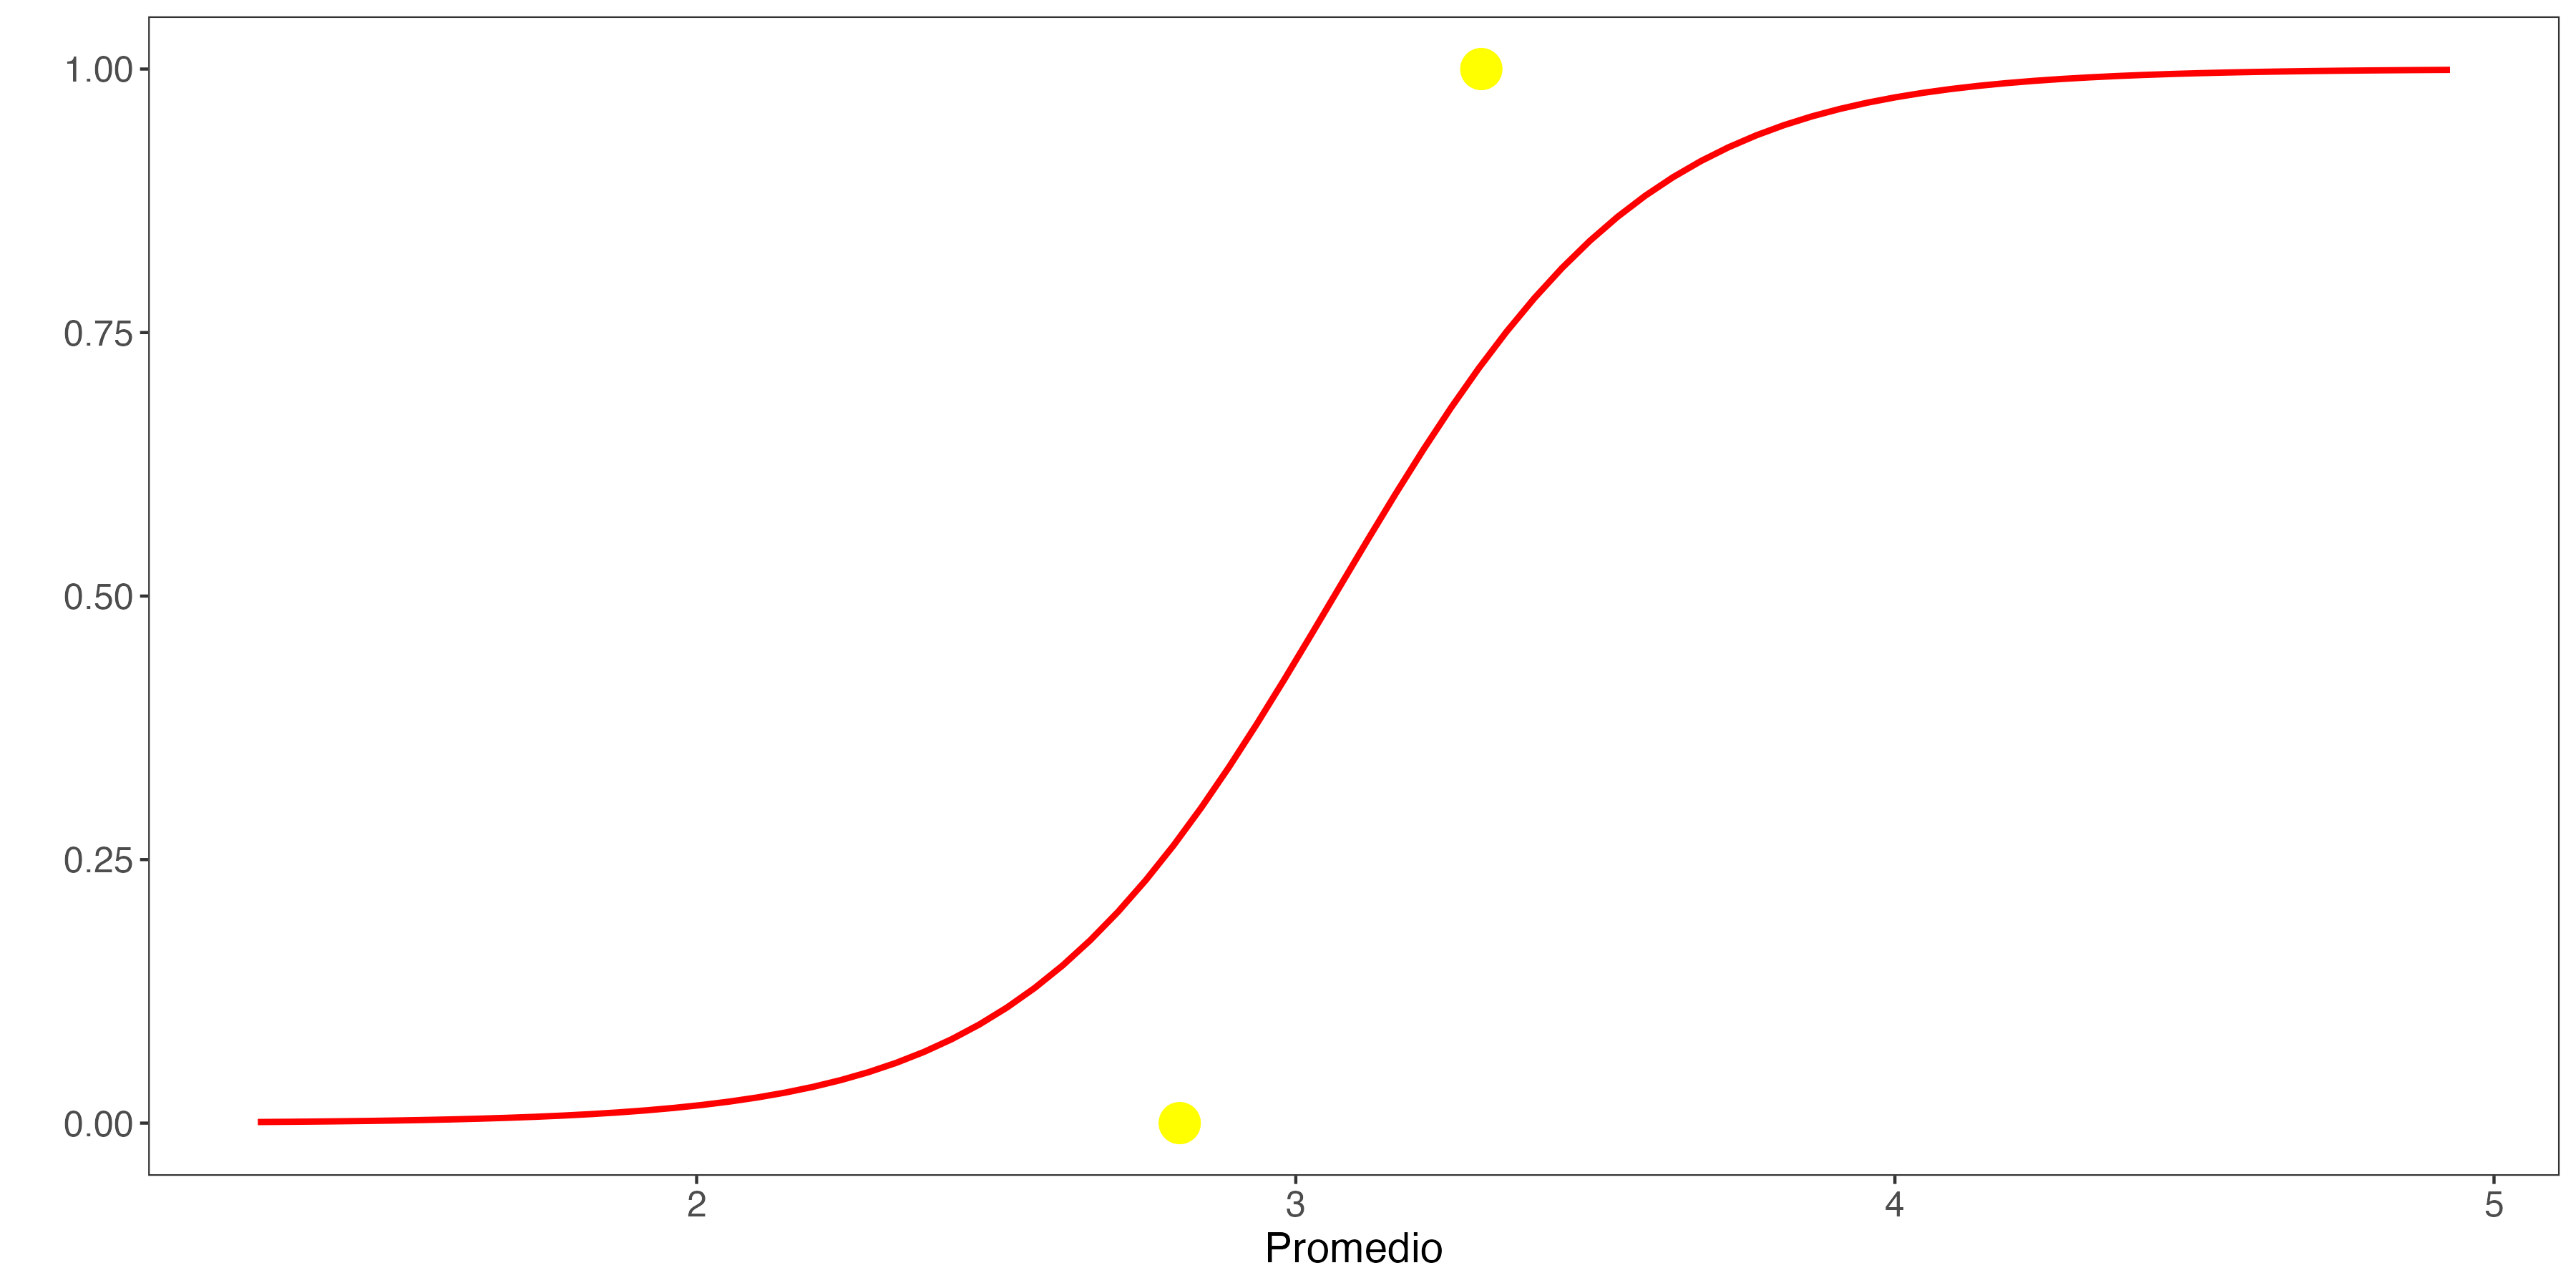
\includegraphics[scale=0.45]{figures/fig4}
              
 \end{figure}



\end{frame}
%----------------------------------------------------------------------%
\begin{frame}[fragile]
\frametitle{Logit}



        \begin{figure}[H] \centering
            \captionsetup{justification=centering}
              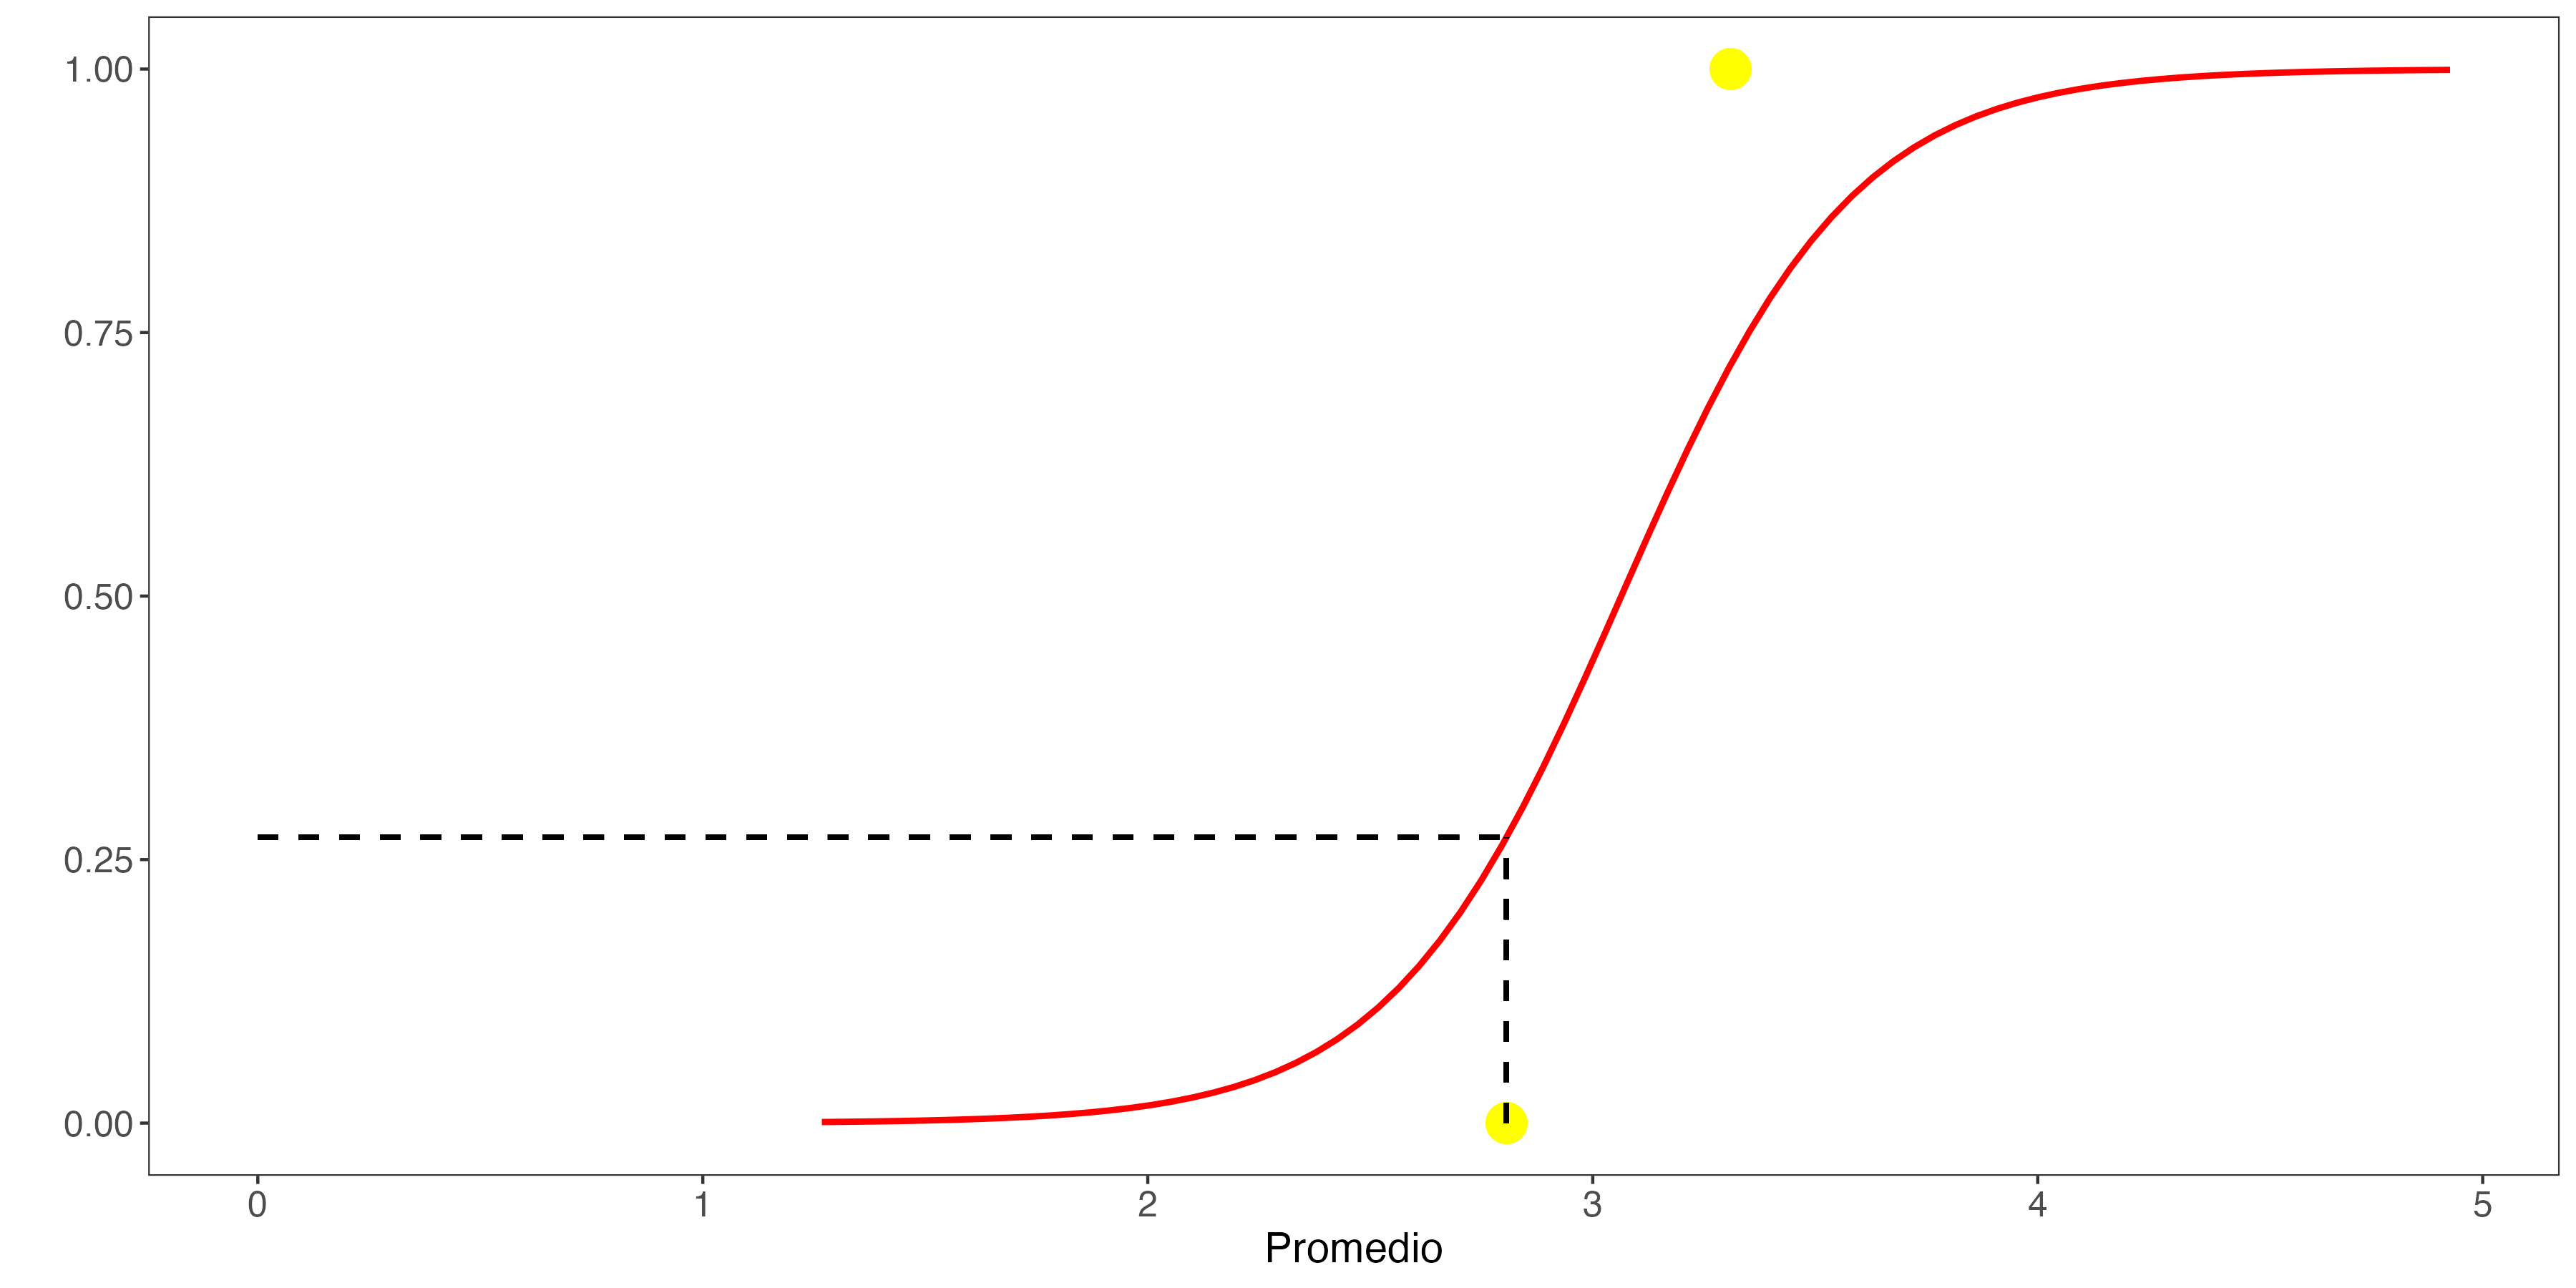
\includegraphics[scale=0.45]{figures/fig5}
              
 \end{figure}


\end{frame}
%----------------------------------------------------------------------%
\begin{frame}[fragile]
\frametitle{Logit}



        \begin{figure}[H] \centering
            \captionsetup{justification=centering}
              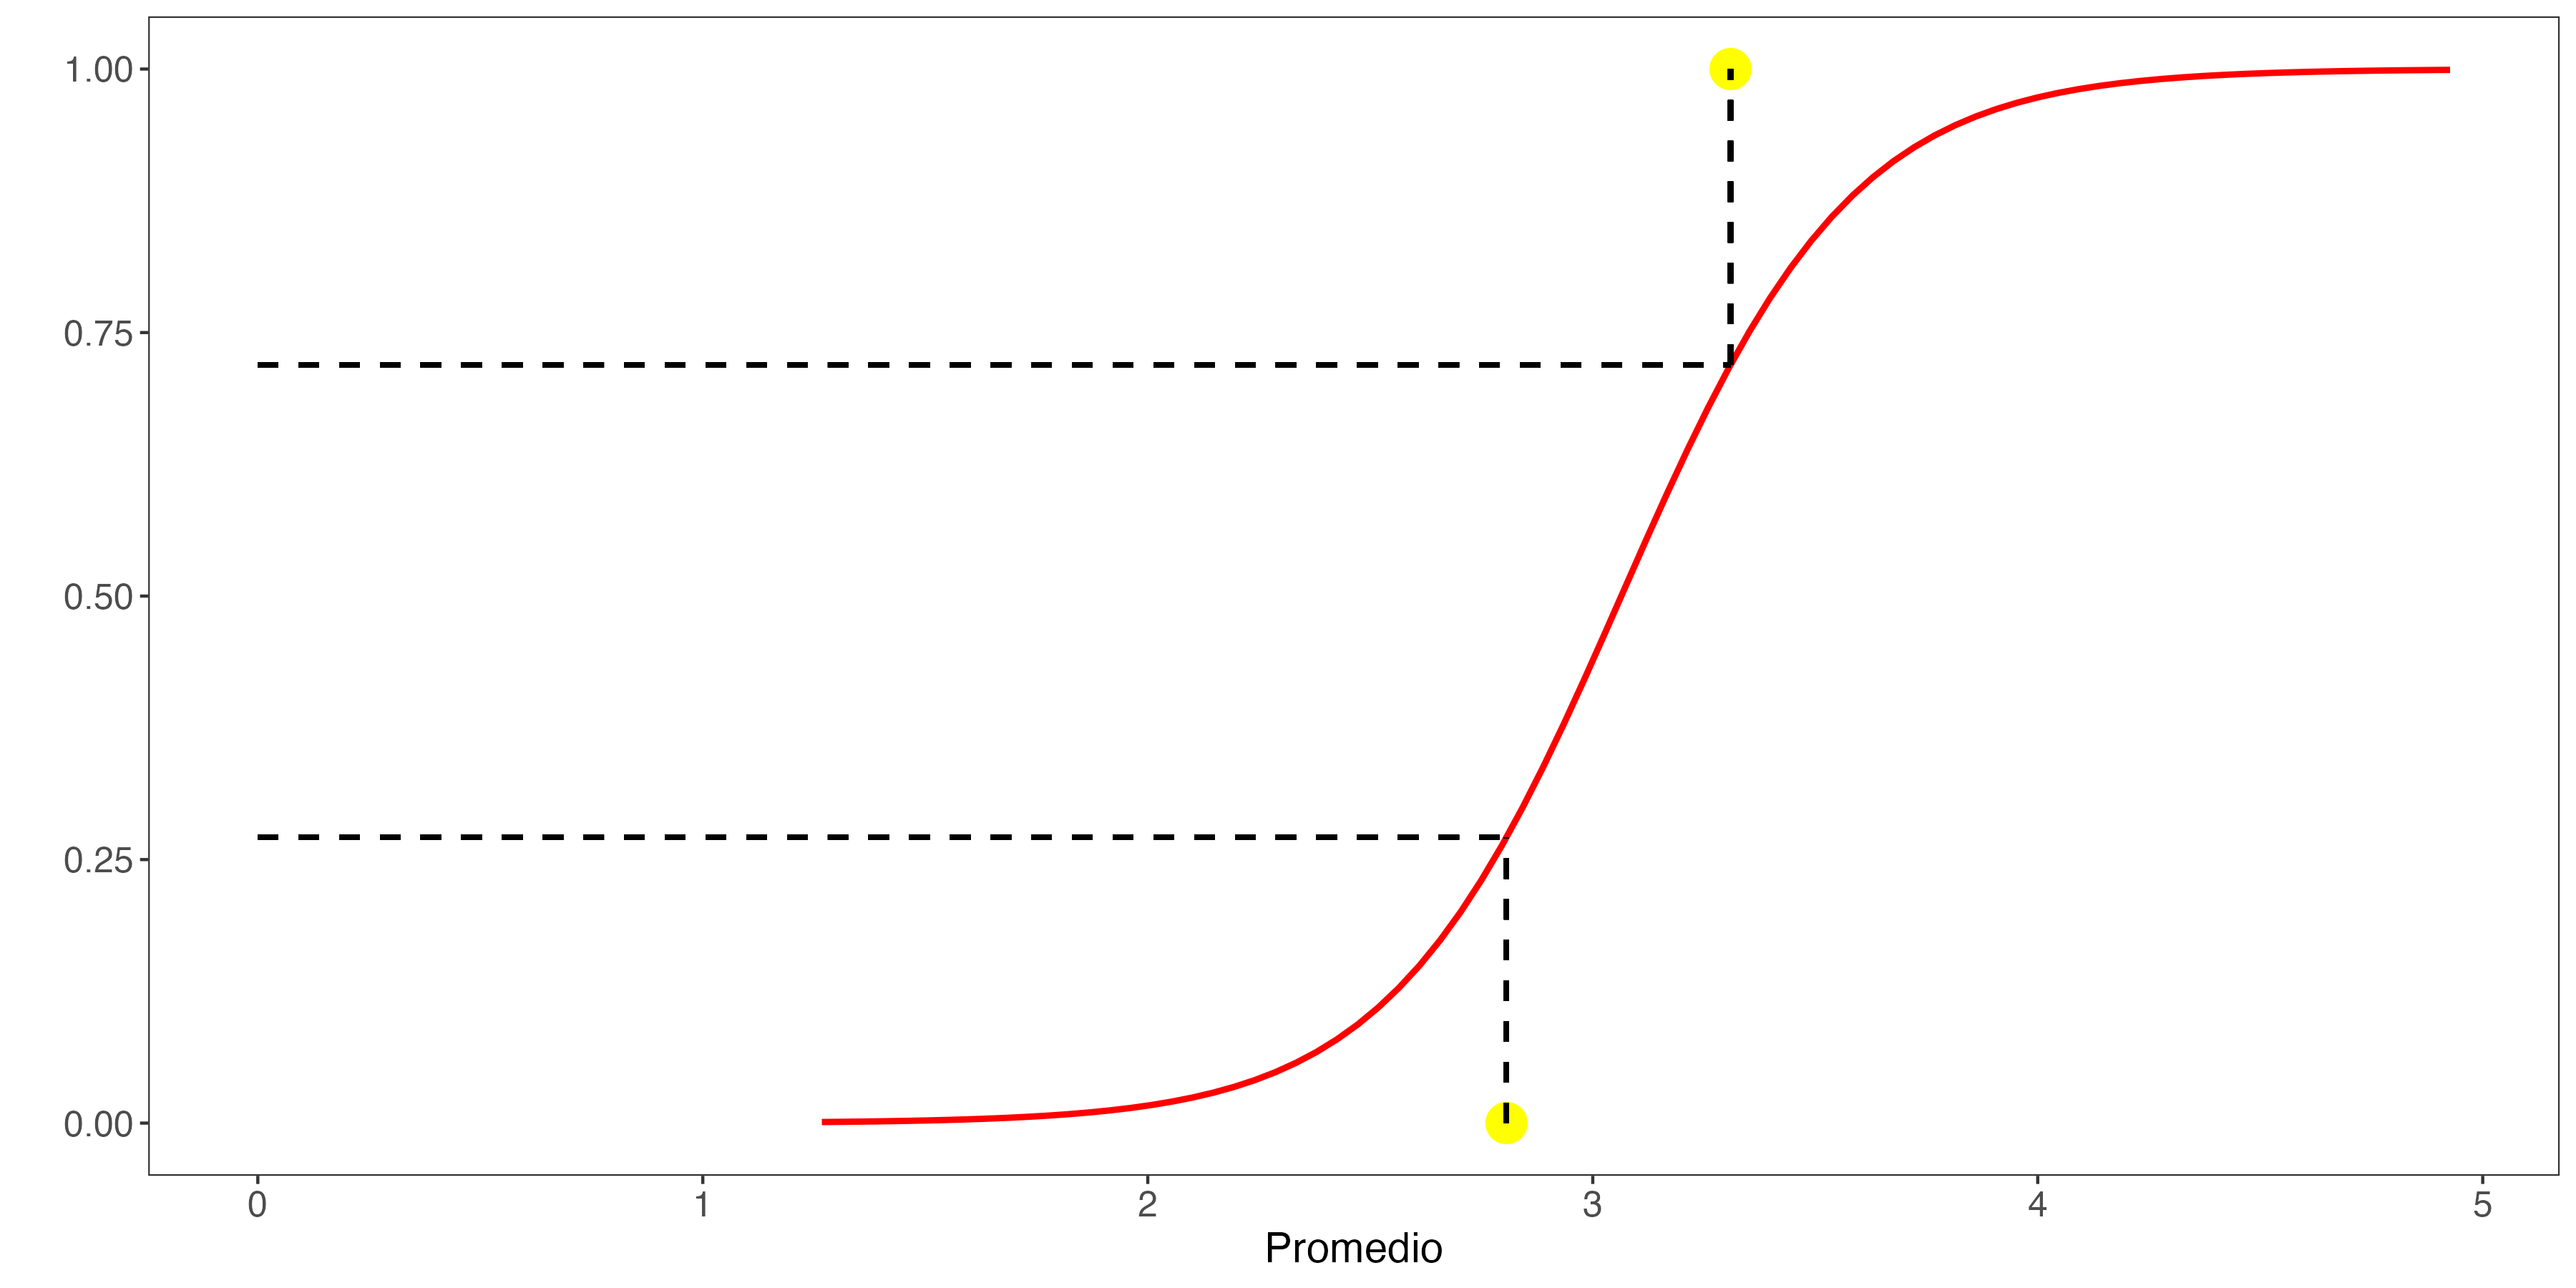
\includegraphics[scale=0.45]{figures/fig6}
              
 \end{figure}


\end{frame}
%----------------------------------------------------------------------%
\begin{frame}[fragile]
\frametitle{Logit}

\begin{itemize}
\item Logit
\begin{align}
p &=\frac{e^{X\beta}}{1+e^{X\beta}} \\ \nonumber
          &=\frac{exp(\beta_0 +\beta_1 x_1 + \dots +\beta_k x_k)}{1+exp(\beta_0 +\beta_1 x_1 + \dots +\beta_k x_k)}
\end{align}

\pause
\item Odds ratio

\begin{align}
ln\left( \frac{p}{1-p}\right) &=X\beta  \\ \nonumber
          &=\beta_0 +\beta_1 x_1 + \dots +\beta_k x_k
\end{align}
\end{itemize}
\end{frame}

%----------------------------------------------------------------------%
%----------------------------------------------------------------------%
\subsection{MLE}
%----------------------------------------------------------------------%
%----------------------------------------------------------------------%

\begin{frame}[fragile]
\frametitle{Aside: Maximum Likelihood Estimation}

\begin{itemize}
    
    \item Developed by Ronald A. Fisher (1890-1962)
    \bigskip
    \item ``If Fisher had lived in the era of ``apps,'' maximum likelihood estimation might have made him a billionaire'' (Efron and Tibshiriani, 2016)
    \bigskip
    \item  Why? MLE gives ``automatically''
    \begin{itemize}    
      \bigskip
      \item Consistent 
      \medskip
      \item Asymptotically normal
      \medskip
      \item  Asymptotically efficient
    \end{itemize} 
\end{itemize}
 
\end{frame}
%----------------------------------------------------------------------%

\begin{frame}[fragile]
\frametitle{Aside: Maximum Likelihood Estimation}

\begin{align}
Pr(Y=y|X) = f(y;\theta)
\end{align}
\begin{itemize}
\item $f()$ known
\medskip
\item $\theta$ unknown
\medskip
\item Example:

\begin{align}
Y|X \sim Poisson(\lambda)
\end{align}
\begin{align}
f(y;\lambda) = \frac{e^{-\lambda} \lambda^y}{y!} 
\end{align}
\end{itemize}



\end{frame}
%----------------------------------------------------------------------%

\begin{frame}[fragile]
\frametitle{Aside: Maximum Likelihood Estimation}

\begin{itemize}
\item $Y_1,\dots,Y_n\sim_{iid}f(Y;\theta)$

\begin{align}
Pr(Y_i =y_i | X_i) =f(y_i;\theta)
\end{align}

\item Likelihood

\begin{align}
L(\theta;y_i)=f(y_i;\theta)
\end{align}
\end{itemize}

 \end{frame}
%----------------------------------------------------------------------%
\begin{frame}[fragile]
\frametitle{Aside: Maximum Likelihood Estimation}

\begin{itemize}
\item For a random sample $y_1,\dots,y_n\sim_{iid}f(y_i;\theta)$
\medskip
\item The likelihood function is



\begin{align}\label{eq:1}
L(\theta|y_1,\dots,y_n) &= \Pi_{i=1}^n L(\theta;y_i) \\ \nonumber
                        &=\Pi_{i=1}^n f(x_i;\theta)
\end{align}

\item A maximum likelihood estimator of the parameter $\theta$:

\begin{align}
\hat \theta^{MLE}=\underset{\theta \in \Theta}{argmax}\, L(\theta,x)
\end{align}
\end{itemize}


 \end{frame}
%----------------------------------------------------------------------%

\begin{frame}[fragile]
\frametitle{Aside: Maximum Likelihood Estimation}

\begin{itemize}
\item Note that maximizing \eqref{eq:1} is the same as maximizing

\begin{align}\label{eq:2}
l(\theta;y_1,\dots,y_n)=\ln L(\theta;y_1,\dots,y_n)=\sum_{i=1}^n l(\theta;y_i)
\end{align}


\item Advantages of \eqref{eq:2}
\medskip
\begin{itemize}
\item Contribution of observation $i$:  $l_i(x|\theta)=\ln f(y_i;\theta)$
\medskip
\item Eq. \eqref{eq:1} is  prone to underflow. 
\end{itemize}
\end{itemize}


\end{frame}
%----------------------------------------------------------------------%
\begin{frame}[fragile]
\frametitle{MLE Logit}
\begin{itemize}
\item Imagine that we have a sample of iid observations $(y_i,x_i)$; $i=1,\dots,n$, where $y_i\in\{0,1\}$
\medskip
\item Under logit we have
\begin{align}
p &=\frac{e^{x_i\beta}}{1+e^{x_i\beta}}
\end{align}
\item Then the likelihood
\begin{align}
L(\theta;y_1,\dots,y_n) &=\Pi_{y_i=1}p_i\Pi_{y_i\neq1}(1-p_i) \\
                        &=\Pi^n_{i=1}p_i^{y_i}(1-p_i)^{1-y_i} \\
                        &=\Pi^n_{i=1}\left(\frac{p_i}{1-p_i}\right)^{y_i}(1-p_i)
\end{align}

\end{itemize}

\end{frame}
%----------------------------------------------------------------------%
\begin{frame}[fragile]
\frametitle{MLE Logit}


\begin{itemize}
  \item The log likelihood is then

\begin{align}
l(\theta;y_1,\dots,y_n)=\sum^n_{i=1}log\left(\frac{p_i}{1-p_i}\right)^{y_i}+\sum^n_{i=1}log(1-p_i)
\end{align}
\item FOC
\begin{align}
\frac{\partial l}{\partial\beta_{j}}&=\sum_{i=1}^{n}\frac{y_{i}}{p_{i}(1-p_{i})}\frac{\partial p_{i}}{\partial\beta_{j}}-\sum_{i=1}^{n}\frac{1}{(1-p_{i})}\frac{\partial p_{i}}{\partial\beta_{j}} \\
&=\sum_{i=1}^{n}\frac{y_{i}-p_{i}}{p_{i}(1-p_{i})}\frac{\partial p_{i}}{\partial\beta_{j}}
\end{align}



  \footnotesize
  \item Note:
  \begin{itemize}
    \footnotesize
    \item This is a system of $K$ non linear equations with $K$ unknown parameters. 
    \item We cannot explicitly solve for $\hat \beta$
    \item It's important to check SOC
  \end{itemize}
\end{itemize}
\end{frame}

%----------------------------------------------------------------------%
\begin{frame}[fragile]
\frametitle{Summary}

\begin{itemize}
  \item We observe $(y_i,X_i)$ $i=1,\dots,n$
  \medskip
  \item Logit


\begin{align}
p_i &=\frac{e^{X_i\beta}}{1+e^{X_i\beta}}
\end{align}

\item Prediction


\begin{align}
\hat{p}_i &=\frac{e^{X_i\hat{\beta}}}{1+e^{X_i\hat{\beta}}}
\end{align}
\item Classification 

\begin{align}
\hat{Y}_i= 1[\hat{p}_i >0.5]
\end{align}
\end{itemize}
\end{frame}
%----------------------------------------------------------------------%
\begin{frame}[fragile]
\frametitle{Example}
\begin{figure}[H] \centering
  \centering
  
\includegraphics[scale=0.35]{figures/baticomputer_meme.jpg}
  \\
  \tiny photo from \url{https://www.dailydot.com/parsec/batman-1966-labels-tumblr-twitter-vine/}
\end{figure}


\end{frame}

%----------------------------------------------------------------------%
%----------------------------------------------------------------------%
\end{document}
